%%%%%%%%%%%%%%%%%%%%%%%%%%%%%%%%%%%%%%%%%%%%%%%%%%%%%%%%%%%%%%%%%%%%%%%%%%%%%%%%%
% Should be compiled with 'pdflatex -jobname="STUDIENUUMMER_FULLNAME" main.tex' %
% REMEMBER TO REMOVE 'CheatSheet' BEFORE HANDING IN                             %
%%%%%%%%%%%%%%%%%%%%%%%%%%%%%%%%%%%%%%%%%%%%%%%%%%%%%%%%%%%%%%%%%%%%%%%%%%%%%%%%%







\documentclass{article}
\usepackage[utf8]{inputenc}
\usepackage{algorithm}
\usepackage{algorithmic}
\usepackage{amsmath}
\usepackage{amssymb}
\usepackage{enumitem}
\usepackage{caption}
\usepackage[parfill]{parskip}
\usepackage{comment}
\usepackage{graphicx}
\usepackage{tikz}
\usepackage{semantic}
\usetikzlibrary{automata, positioning, arrows}
\tikzset{
    ->,
    node distance=3cm, 
    every state/.style={thick, fill=gray!10}
}


\DeclareCaptionType{equ}[Equation][List of Equations]
\DeclareCaptionListFormat{equ}{%
    #1 #2
}
\DeclareCaptionLabelFormat{equ}
{%
    #1 #2:
}
\DeclareCaptionLabelSeparator{equ}{}
\DeclareCaptionFormat{equ}
{%
    \textbf{#1#2}#3
}
\captionsetup[equ]
{
    format=equ,
    labelformat=equ,
    listformat=simple,
    skip=-5pt,
    labelsep=equ,
}

\newcommand{\floor}[1]{\left\lfloor{#1}\right\rfloor}
\newcommand{\ceil}[1]{\left\lceil{#1}\right\rceil}

\title{Syntax and Semantics Exam}

\author{NAME}
\date{June 2022}

\makeatletter
\AtBeginDocument{\let\c@equation\c@equ}
\makeatother

\begin{document}

\maketitle

\section*{Symbol Cheat Sheet}

\begin{tabular}{|c|c|} \hline
    \textbf{Comment}    & \textbf{Symbol} \\ \hline
    Not                 & $\neg$ \\ \hline
    Not less than       & $\not<$ \\ \hline
    Not greater than    & $\not>$ \\ \hline
    Not less than       & $\leq$ \\ \hline
    Not less than       & $\geq$ \\ \hline
    Not equal           & $\neq$ \\ \hline
    Similar             & $\sim$ \\ \hline
    Similar or equal    & $\simeq$ \\ \hline
    Approx              & $\approx$ \\ \hline
    Subset              & $\subset$ \\ \hline
    Not subset          & $\not\subset$ \\ \hline
    Subset Equal        & $\subseteq$ \\ \hline
    Not Subset Equal    & $\not\subseteq$ \\ \hline
    Bum                 & $\vdash$ \\ \hline
    Is member of        & $\in$ \\ \hline
    Is not member of    & $\notin$ \\ \hline
    Times               & $\cdot\text{ }\times$ \\ \hline
    Empty set           & $\emptyset$ \\ \hline
    Nothing             & $\varnothing$ \\ \hline
    Number Sets         & $\mathbb{N}\text{ }\mathbb{Z}\text{ }\mathbb{Q}\text{ }\mathbb{R}\text{ }$ \\ \hline
    Union/Intersect     & $\cup\text{ }\cap$ \\ \hline
    Logical and/or      & $\lor\text{ }\land$ \\ \hline
    For all/ Exists     & $\forall\text{ }\exists$ \\ \hline
    Segment             & $\overline{\rm AB}$ \\ \hline
    Angle Brackets      & $\langle\text{ }\rangle$ \\ \hline
    Maps to             & $\mapsto\text{ }\longmapsto$ \\ \hline
    Arrows              & $\rightarrow\text{ }\leftarrow\text{ }\longrightarrow\text{ }\Rightarrow$ \\ \hline
    Epsilon             & $\epsilon\text{ }\varepsilon$ \\ \hline
    Sigma               & $\Sigma$ \\ \hline
    delta               & $\delta$ \\ \hline
    Gamma               & $\Gamma$ \\ \hline
\end{tabular}


\section*{Syntax}


\begin{figure}[H]
    \centering 
    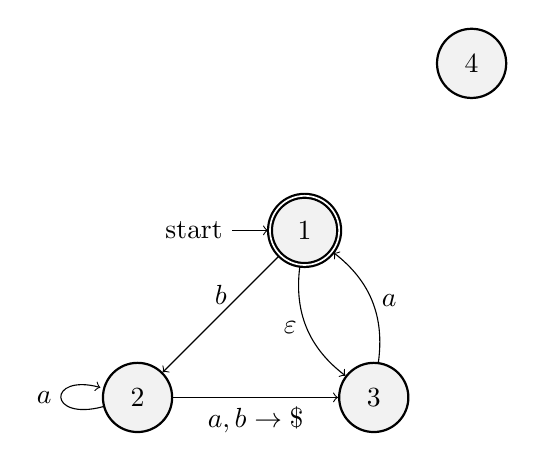
\begin{tikzpicture}
        \node[state, initial, accepting] (1) {$1$};
        \node[state, below left of=1] (2) {$2$};
        \node[state, right of=2] (3) {$3$};
        \node[state, above right of=1] (4) {$4$};
        \draw (1) edge[above] node{$b$} (2)
        (1) edge[below, bend right, left=0.3] node{$\varepsilon$} (3)
        (2) edge[loop left] node{$a$} (2)
        (2) edge[below] node{$a, b \rightarrow \$$} (3)
        (3) edge[above, bend right, right=0.3] node{$a$} (1);
    \end{tikzpicture}
    \caption{Caption of the Figure}
    \label{fig:label}
\end{figure}
\section*{Semantics}
\begin{equ}[H]
    \begin{align*}
        [ASS_{BSS}] \quad & env_V, env_P \vdash \langle x := a, sto\rangle \rightarrow a sto[l\rightarrow v]\\
        & \text{where } env_V, sto \vdash a \rightarrow_a v\\
        & \text{and } env_V x = l\\ \\
        [WHILE\text{-}TRUE_{BSS}] \quad & \inference{ env_V, env_P \vdash \langle S,sto\rangle\rightarrow sto''\\env_V, env_P \vdash \langle\texttt{while $b$ do $S$}, sto''\rangle \rightarrow sto'}{ env_V, env_P \vdash \langle\texttt{while $b$ do $S$}, sto\rangle \rightarrow sto'}\\
        & \text{if } env_V, sto \vdash b \rightarrow_b tt = env_V(next) \\\\
        [IF\text{-}TRUE_{BSS}] \quad & \inference{env_V, env_P \vdash \langle S_1,sto\rangle \rightarrow sto'}{env_V, env_P \vdash \langle\texttt{if $b$ then $S_1$ else $S_2$} \rangle \rightarrow sto'}\\
        & \text{if } env_V, sto \vdash b \rightarrow_b tt = env_V(next) \\\\
        [VAR_{EXP}] \quad & \inference{E(x)=T}{E\vdash x:T}\\\\
        [ADD\text{-}NUMBER_{EXP}] \quad & \inference{E \vdash e_{1}\texttt{:number} \quad E \vdash e_{2}\texttt{:number}}{E \vdash e_{1} + e_{2} \texttt{:number} }& \\\\
        [AND_{EXP}] \quad & \inference{E \vdash e_{1} \texttt{:bool}\quad E \vdash e_{2} \texttt{:bool}}{E \vdash e_1 \&\& e_2 :\texttt{bool}}
    \end{align*}
    \caption{Caption of Equation}
    \label{equ:label}
\end{equ}

Other equation:
\begin{equation}
    [ADD\text{-}NUMBER_{EXP}] \quad \inference{a1 \rightarrow v1 \quad a2 \rightarrow v2}{a1+a2=v} \quad \text{where } v = v1 + v2
    \label{equ:other_equation}
\end{equation}
 %%%%% REMEMBER TO REMOVE THIS BEFORE HANDING IN
\section*{Question 1}

\subsection*{A}

\subsection*{B}

\section*{Question 2}

\section*{Question 3}

\section*{Question 4}


\end{document}
